\chapter{Diseño e implementación} % Main chapter title

En este capítulo se explican las consideraciones de diseño realizadas al elaborar el hardware del dispositivo. También se dan detalles de la implementación del software que usa el dispositivo y finaliza con la documentación elaborada.
\label{Chapter3} 

%----------------------------------------------------------------------------------------
%	SECTION 1
%----------------------------------------------------------------------------------------
\section{Desarrollo de \textit{hardware}}
 
\subsection{Estructura Planteada }

Se comenzó a diseñar el circuito esquemático del hardware teniendo como punto de partida el microcontrolador a utilizar y planteando cómo se debería comunicar este con el circuito integrado de medición. Luego teniendo en cuenta un diagrama de bloques previamente realizado (este puede observarse en la figura \ref{fig:bloquess1}), se decidió que la placa debería poseer dos sectores aislados eléctricamente entre si. Un sector sería destinado exclusivamente para las mediciones de altas tensiones y el otro sector sería destinado al microcontrolador.

En el sector del microcontrolador se encontrarían, además del microcontrolador principal, los integrados de comunicación y las salidas.
Por otro lado el sector de medición debía manejar alta tensión, por lo que allí irían los arreglos analógicos para lograr la medición. 

También se tuvo en cuenta la condición de que el PCB (\textit{printed circuit board}) debía poseer las dimensiones mostradas en la figura \ref{fig:medidaspcb}, que son las necesarias para insertar la placa en una carcasa estándar, de uso habitual por la empresa.

\begin{figure}[!htb]
	\centering
	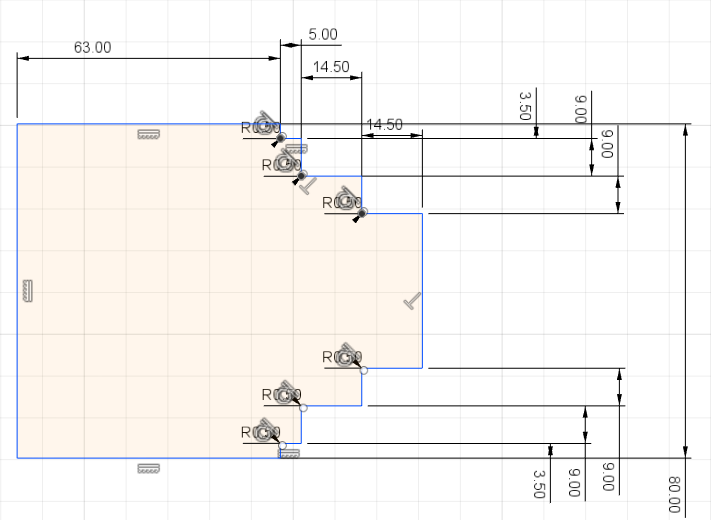
\includegraphics[width=110mm,keepaspectratio]{Figures/Placa1v6.png}
	\caption{Medidas de la placa electrónica.}
	\label{fig:medidaspcb}
\end{figure}

Una vez que fueron establecidas las medidas y los conexionados de comunicación que debería tener el microcontrolador, se delimitó la placa en los dos sectores previamente mencionados. Esta división puede observarse en la figura \ref{fig:pcbbase}, ambas divisiones deberían encontrarse aisladas, por lo que se debía dejar cierto espacio entre las pistas de cobre de cada sector.

\begin{figure}[!htb]
	\centering
	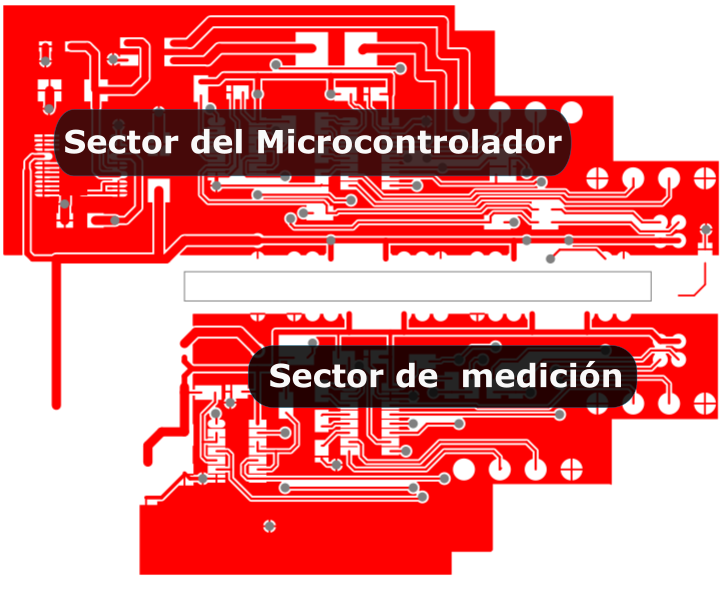
\includegraphics[width=80mm,keepaspectratio]{Figures/esquema22.png}
	\caption{Placa de ejemplo para la aislación.}
	\label{fig:pcbbase}
\end{figure}



La figura \ref{fig:pcbbase} es una vista de un diseño de otro proyecto electrónico que proveyó la empresa como punto de partida para el desarrollo de los circuitos impresos.

Se estableció entonces que en el sector del microcontrolador se encontrarán los puertos de comunicación y en el sector de medición, los integrados y circuitos analógicos que adapten las entradas a medir.

\subsection{Componentes esenciales}

Basándose en los requerimientos se fue definiendo al dispositivo como  un conjunto de circuitos, estos son:

\begin{itemize}
\item un circuito de alimentación.
\item circuito de adaptación de microcontrolador.
\item circuito de aislación o de cambio de nivel.
\item circuito de medición.
\item circuito de comunicación por puerto.
\item circuito de relé.
\item circuito de salida analógica.
\end{itemize}

Todos estos circuitos se encuentran en el sector de microcontrolador que puede verse de la figura \ref{fig:pcbbase}, a excepción del circuito de  medición que se encuentra en el sector de medición  y el circuito de aislación que funciona de interfaz y se encuentra en ambos sectores.

\subsubsection{Circuito de alimentación}
Se comenzó a realizar el circuito teniendo como presupuesto que la alimentación se haría con una fuente alterna de 8 V a 30 V.

Para la alimentación se optó por una fuente switching  LM2574 que provee 5 V a un regulador lineal de 3,3 V necesarios para operar el microcontrolador. El circuito descrito puede observarse en la figura \ref{fig:circalim1}.

\begin{figure}[!htb]
	\centering
	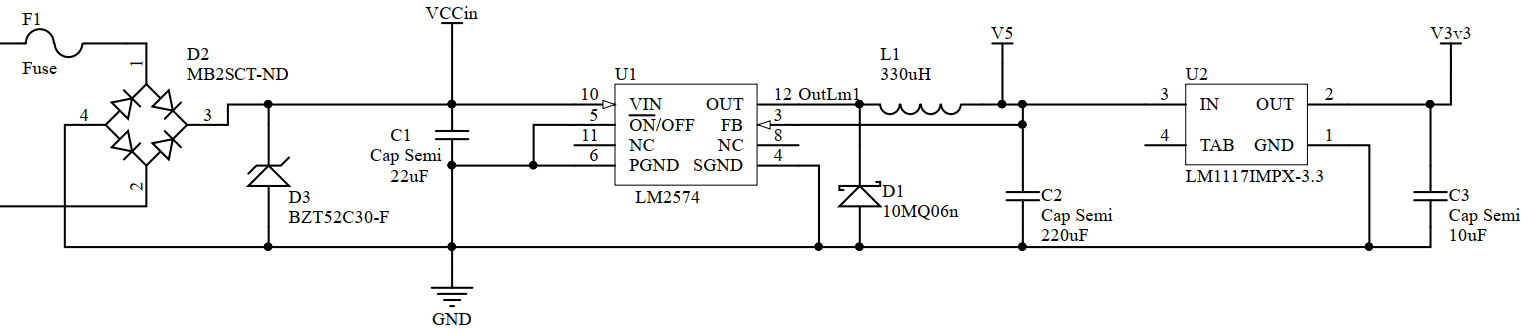
\includegraphics[width=120mm,keepaspectratio]{Figures/alimentacion1.png}
	\caption{Circuito esquemático de la alimentación de la placa.}
	\label{fig:circalim1}
\end{figure}

\subsubsection{Circuito de aislación o de cambio de nivel}
Para proteger al microcontrolador de elevadas tensiones se utilizó un integrado de aislación; para alimentar el circuito de medición, un conversor de continua a continua. También se añadió un aislador digital para comunicar el microcontrolador principal con un integrado de medición.

\begin{figure}[!htb]
	\centering
	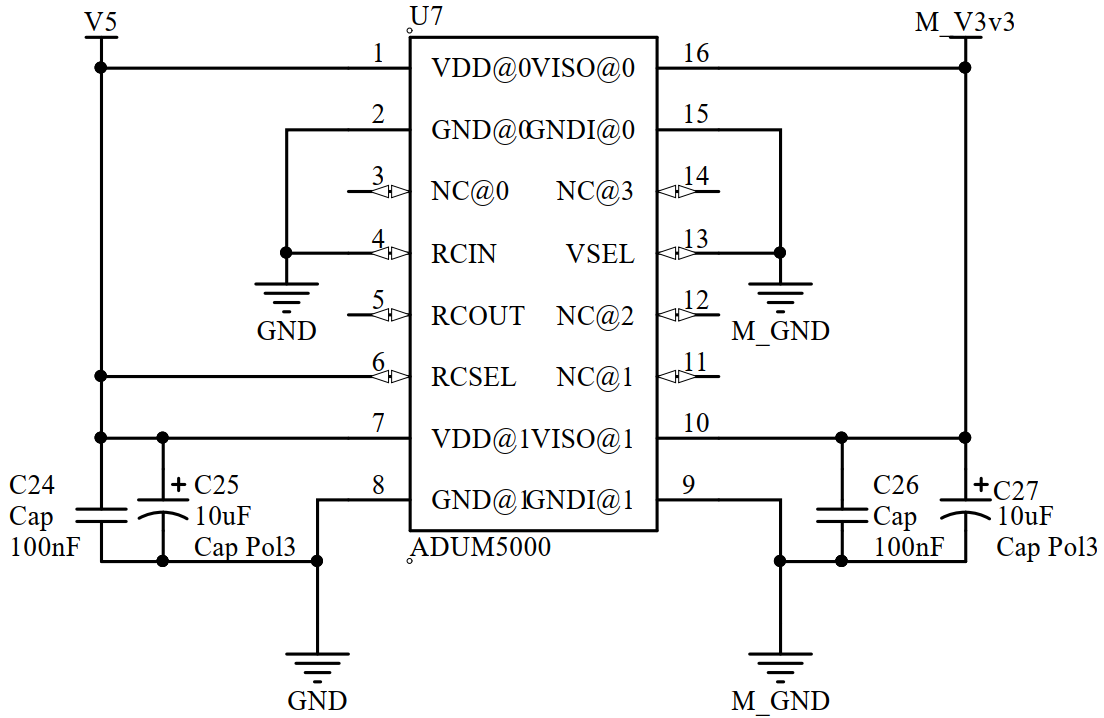
\includegraphics[width=100mm,keepaspectratio]{Figures/alimentacion2.png}
	\caption{Circuito esquemático de la alimentación del sector aislado.}
	\label{fig:circaisl1}
\end{figure}

\begin{figure}[!htb]
	\centering
	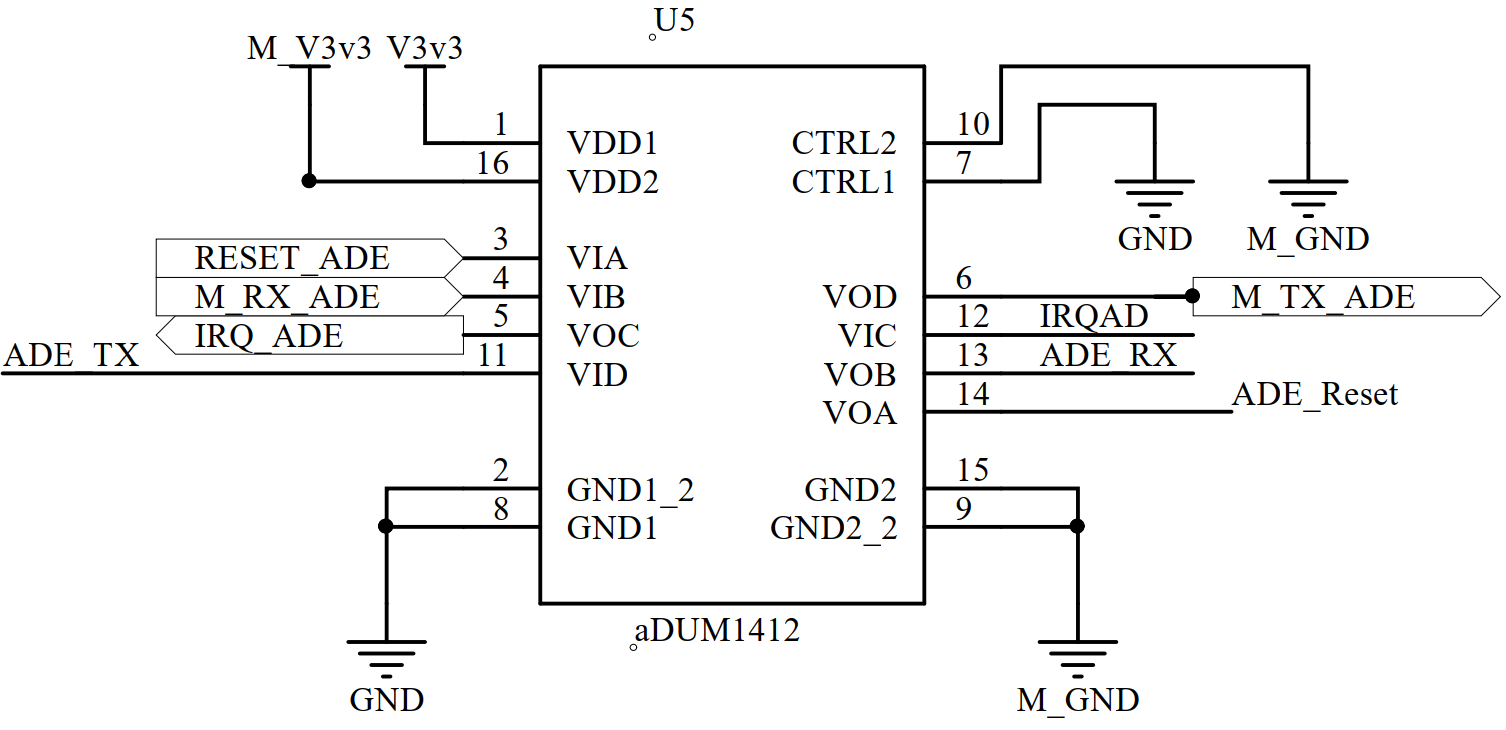
\includegraphics[width=100mm,keepaspectratio]{Figures/comaislado1.png}
	\caption{Circuito esquemático de la comunicacion digital aislada.}
	\label{fig:circaisl2}
\end{figure}

 
\subsubsection{Circuito de adaptación de microcontrolador}

El circuito de adaptación está integrado por resistores y capacitores necesarios para el correcto funcionamiento del microcontrolador, como también un cristal externo para usarlo como oscilador. Se usó un microcontrolador de la familia MSP430 de uso habitual en la empresa. 

En el circuito de adaptación se incluyó un semiconductor para tensión de referencia y un cristal de 32768 Hz. Para el armado del dispositivo se seleccionó el modelo MSP430F2618, que posee un DAC interno de 12 bit que es de utilidad para la salida analógica utilizada en el lazo de corriente.

Para programar al microcontrolador se añadió una conexión JTAG para conectar un programador flash de la empresa Texas Instrument. Este puerto de salida puede verse en la figura \ref{fig:jitag}.

\begin{figure}[!htb]
	\centering
	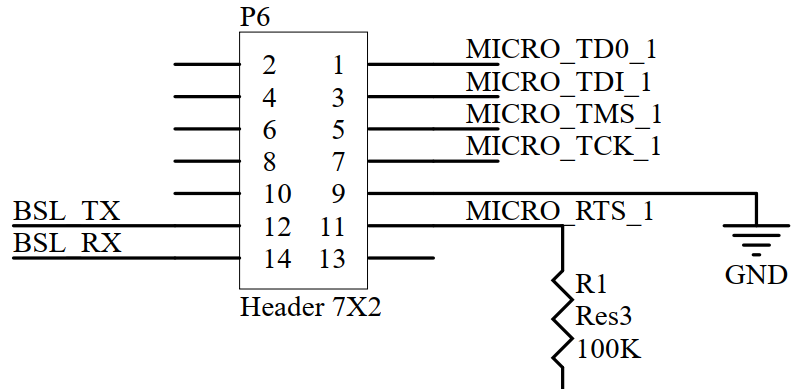
\includegraphics[width=120mm,keepaspectratio]{Figures/JTAG1.png}
	\caption{Header JTAG añadido al PCB.}
	\label{fig:jitag}
\end{figure}

\subsubsection{Circuito de comunicación por puerto}
Como se estableció en los requisitos, se implementaron integrados para la comunicación RS232, un max3222 y para la RS485, un integrado ISL83485. Estos integrados facilitan la adaptación de tensiones para lograr el estándar de comunicación deseado.

\begin{figure}[!htb]
	\centering
	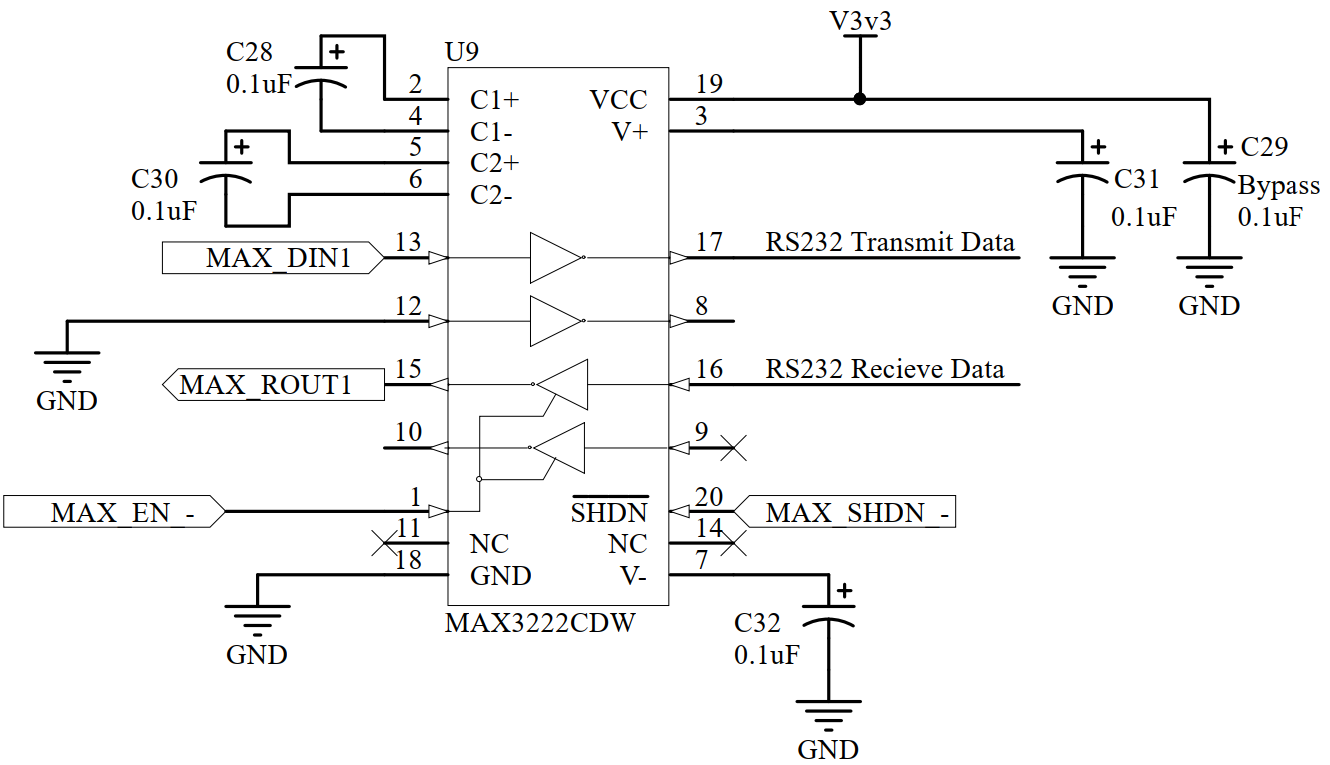
\includegraphics[width=120mm,keepaspectratio]{Figures/RSS232_1.png}
	\caption{Circuito esquemático con la implementación del MAX3222.}
	\label{fig:2321esquem}
\end{figure}

\begin{figure}[!htb]
	\centering
	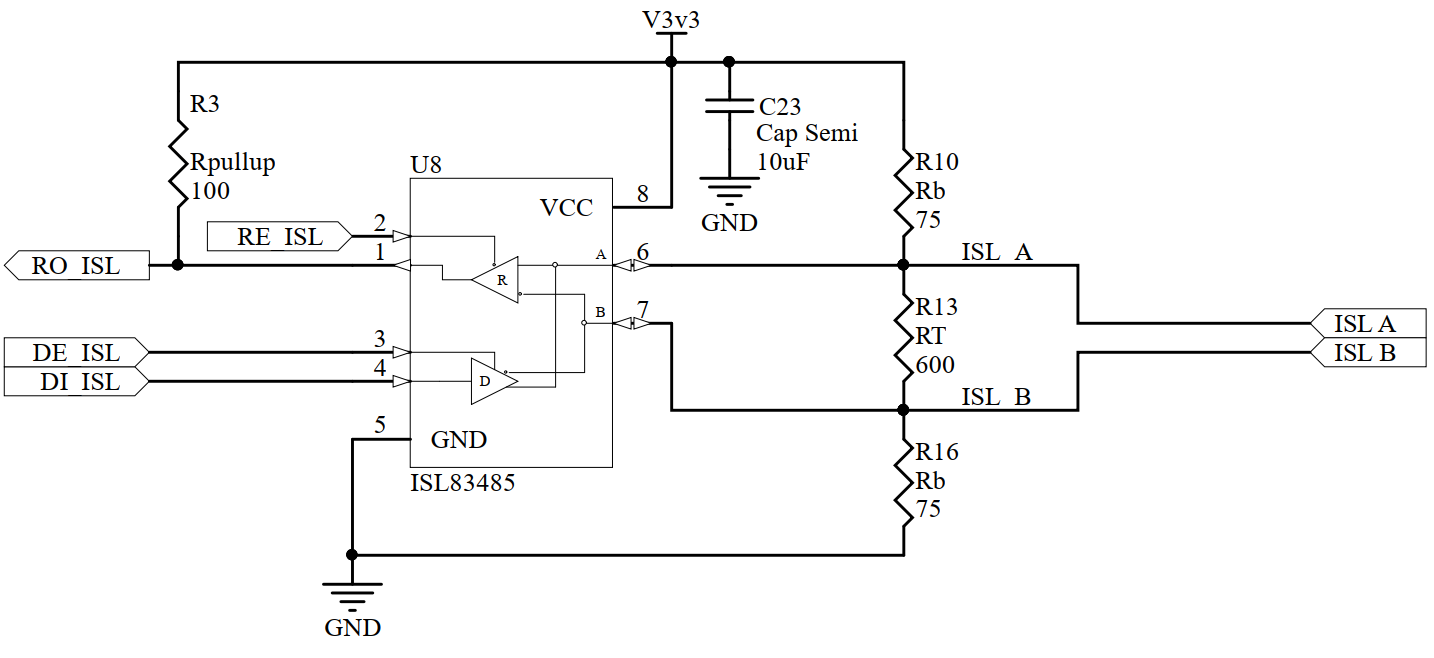
\includegraphics[width=120mm,keepaspectratio]{Figures/RSS485_1.png}
	\caption{Circuito esquemático con la implementación del ISL83485.}
	\label{fig:4851esquem}
\end{figure}


\subsubsection{Circuito de relé}
El circuito es integrado por los componentes mínimos para que el microcontrolador pueda manejar un relé que se acciona con tensiones del orden de los 5 volts. El circuito puede verse en la figura \ref{fig:rele1equem}.

\begin{figure}[!htb]
	\centering
	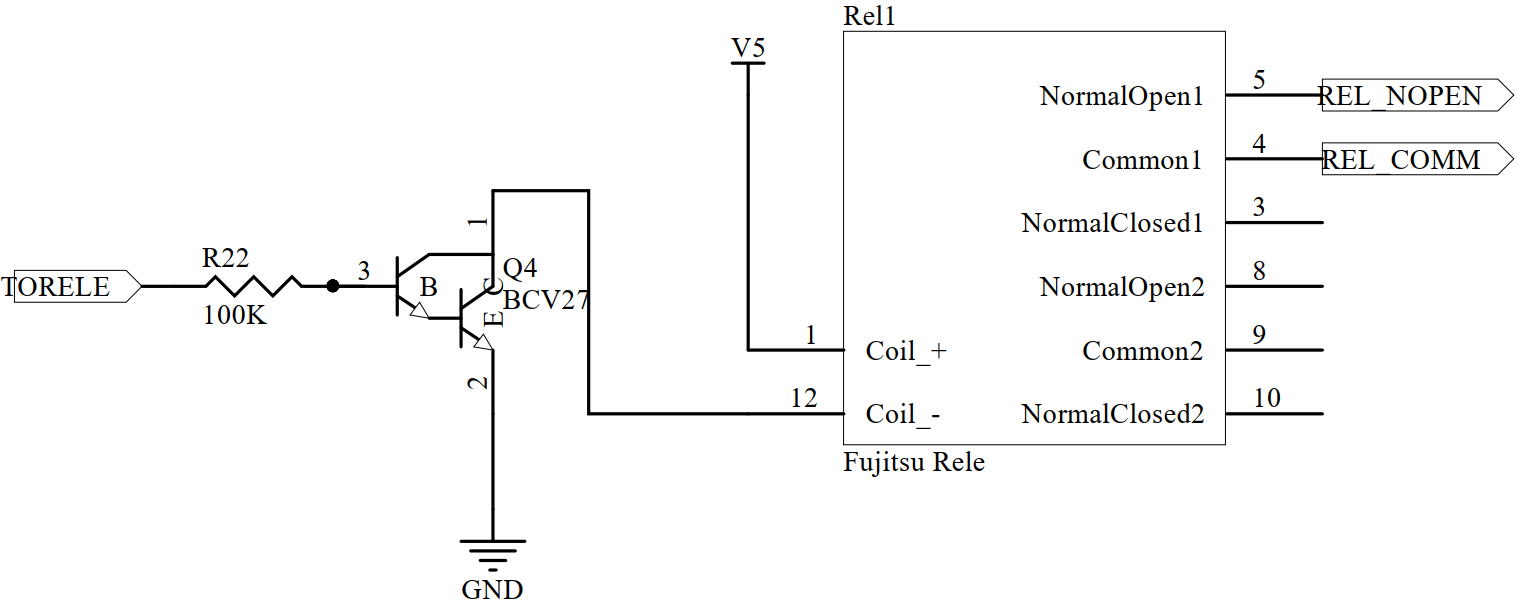
\includegraphics[width=120mm,keepaspectratio]{Figures/rele1.png}
	\caption{Transistor darlington para la acción del relé.}
	\label{fig:rele1equem}
\end{figure}

\subsubsection{Circuito de salida analógica}
Este circuito esta compuesto por un \textit{buffer} combinado con un integrado regulador de corriente para lograr una salida de lazo de corriente 4 - 20 mA.

\begin{figure}[!htb]
	\centering
	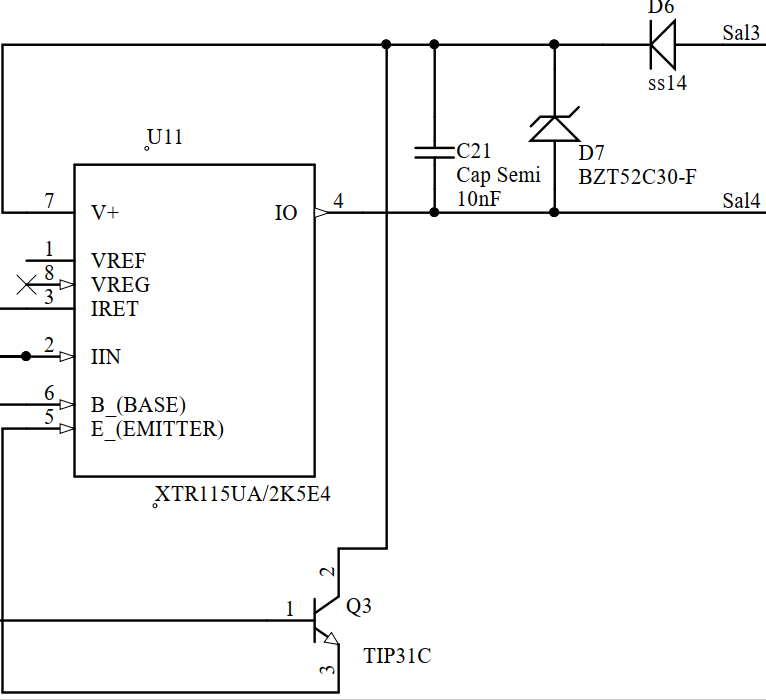
\includegraphics[width=120mm,keepaspectratio]{Figures/salida420.png}
	\caption{Circuito de salida 4 - 20 mA.}
	\label{fig:rele1equem}
\end{figure}


\subsubsection{Circuito de medición}

Para realizar la medición se optó por un integrado multifuncional de medición de una sola fase. El  integrado permitió la rápida implementación de un medidor en el circuito del dispositivo. El integrado elegido es el ADE7953 del fabricante Texas Instrument. El integrado es un SOC (\textit{System on a Chip}) que adapta un AFE (\textit{analog front-end} ) para su fácil uso. El circuito esquemático del ADE7953 puede verse en la  figura \ref{fig:ade79esquem}.

\begin{figure}[!htb]
	\centering
	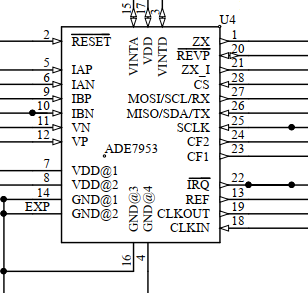
\includegraphics[width=100mm,keepaspectratio]{Figures/ade7953.png}
	\caption{Diagrama de bloque del ADE7953.}
	\label{fig:ade79esquem}
\end{figure}

El integrado de medición puede comunicarse con el microcontrolador a través de tres diferentes protocolos: I2C, SPI y UART, para esto deben realizarse las conexiones necesarias. Debido a la decisión de aislar el integrado y que las condiciones de espacio no permitían sobrepasarse con la cantidad de integrados para aislar, se realizaron las conexiones para la comunicación UART solamente.

\subsection{Esquema analógico de medición }
Como el principal objetivo del dispositivo es medir, se explican de manera muy breve los arreglos analógicos que se implementaron.

Suponiendo que las tensiones a medir fuesen del orden de los 600 V y teniendo en cuenta que la máxima tension que soporta un pin del integrado es de 2 V, se añadió una serie de resistores para lograr 1 M$\Omega$ de resistencia en la entrada de medición, de modo de atenuar la tension. Una vez atenuada la tensión se agregó un divisor resistivo del cual el integrado mide.

\begin{figure}[!htb]
	\centering
	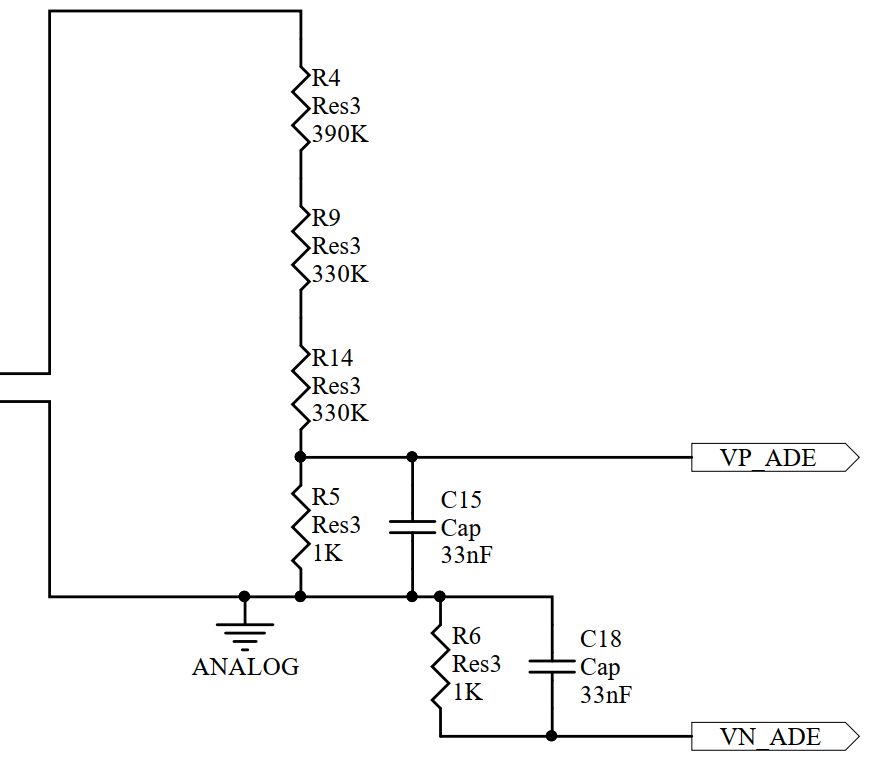
\includegraphics[width=80mm,keepaspectratio]{Figures/medicionvoltaje.png}
	\caption{Circuito esquemático de la entrada de tensión.}
	\label{fig:medvolt}
\end{figure}

Para la medición de corriente es común ver en los módulos comerciales el uso de una bobina de Rogowski, sin embargo para el módulo diseñado se optó por usar un \textit{shunt} para que el dispositivo no dependiera de otro objeto discreto para su instalación. El \textit{shunt} elegido soporta grandes corrientes y se tomaron precauciones en las pistas del PCB para que pudiera operar con normalidad.

\begin{figure}[!htb]
	\centering
	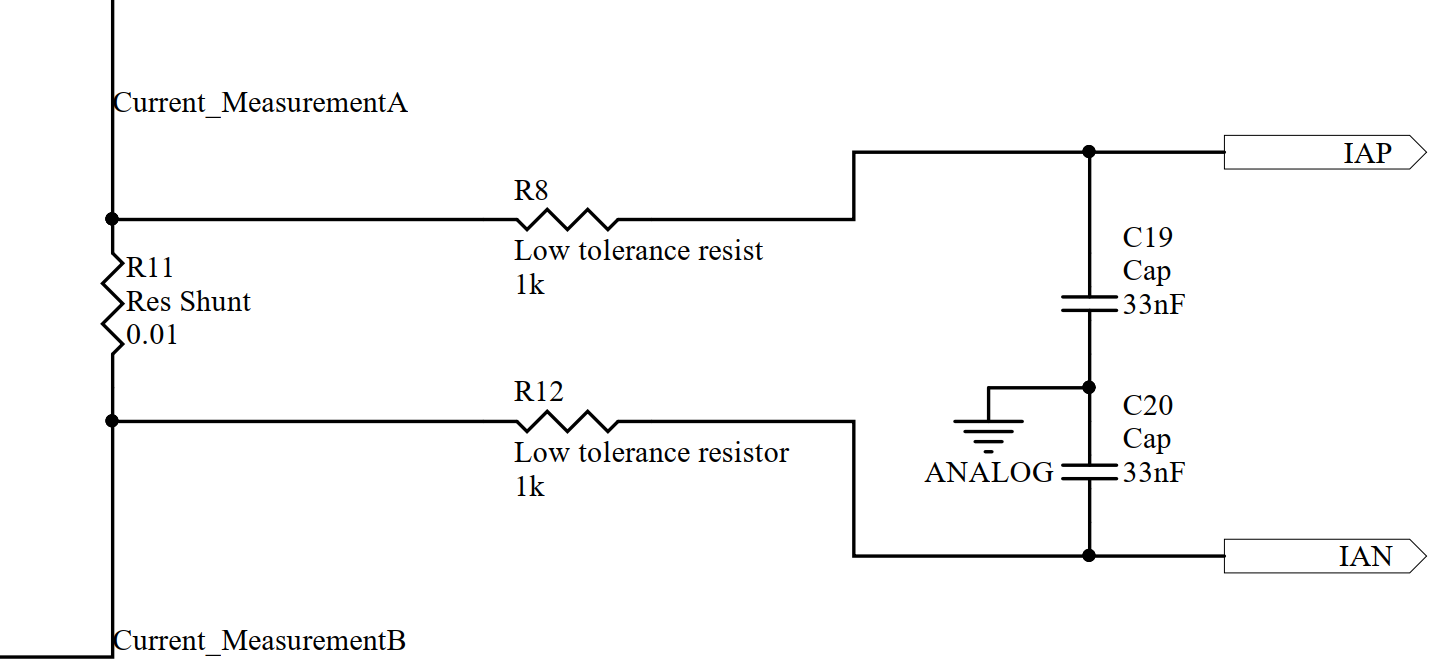
\includegraphics[width=120mm,keepaspectratio]{Figures/medicioncorriente.png}
	\caption{Circuito esquemático de la entrada de corriente.}
	\label{fig:medcurrent}
\end{figure}

\subsection{Fabricación}

Una vez completada la totalidad de las conexiones lógicas en el circuito esquemático, se debía decidir sobre el posicionamiento de los componentes, el tamaño de las perforaciones y la distribución de cada circuito. Se estableció desde la empresa privada que todos los componentes pasivos en lo posible fueran de montaje superficial, por lo que la mayoría de resistores y capacitores serian de encapsulado 0805. 

%Un 0805 puede verse en la figura \ref{fig:smd0805}.

%\begin{figure}[!htb]
%	\centering
%	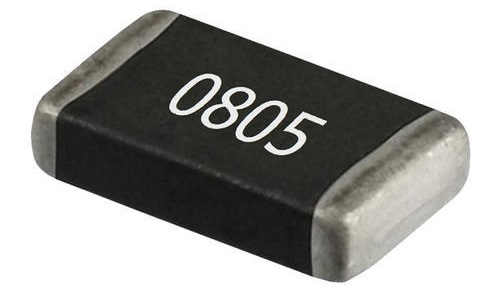
\includegraphics[width=50mm,keepaspectratio]{Figures/smd0805.jpg}
%	\caption{Componente de soldadura superficial.}
%	\label{fig:smd0805}
%\end{figure}

Se dejó espacio para una entrada de conector RJ45 para un futuro puerto LAN Ethernet y se delimitó una zona de exclusión para dividir al PCB en una zona de medición y una zona de microcontrolador.

Debido a que el PCB iba a ser encapsulado por una carcasa de plástico con posibilidad de conexión de 16 salidas, se decidió previamente cómo debería ser el esquema de conexiones. Se dejo un conector de 4 salidas para las mediciones ya que este se encontraría en un nivel aislado.

\begin{figure}[!htb]
	\centering
	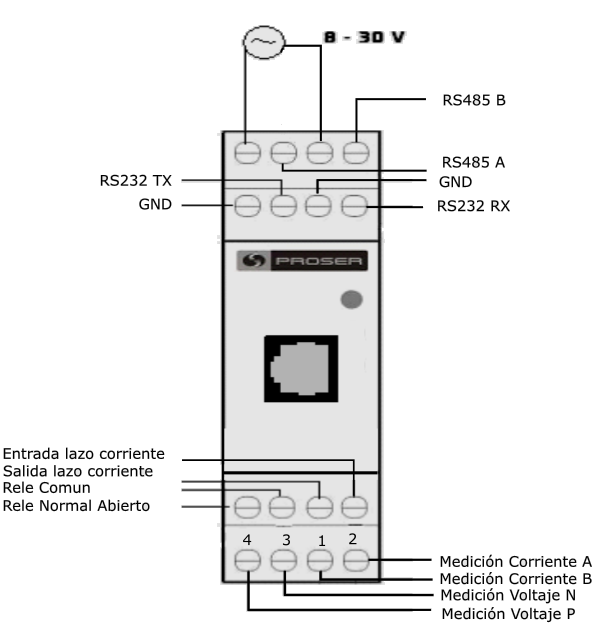
\includegraphics[width=120mm,keepaspectratio]{Figures/conectores2.png}
	\caption{Salidas del dispositivo.}
	\label{fig:salidas01}
\end{figure}

Se decidió fabricar las placas electrónicas en Argentina. La empresa fabricante tiene publicada una tabla donde divulga con qué tipos de tecnología de fabricación trabaja. Se estableció como estándar a usar el de 8 mils y se trabajó con ese limite en el CAD de diseño.

\begin{figure}[!htb]
	\centering
	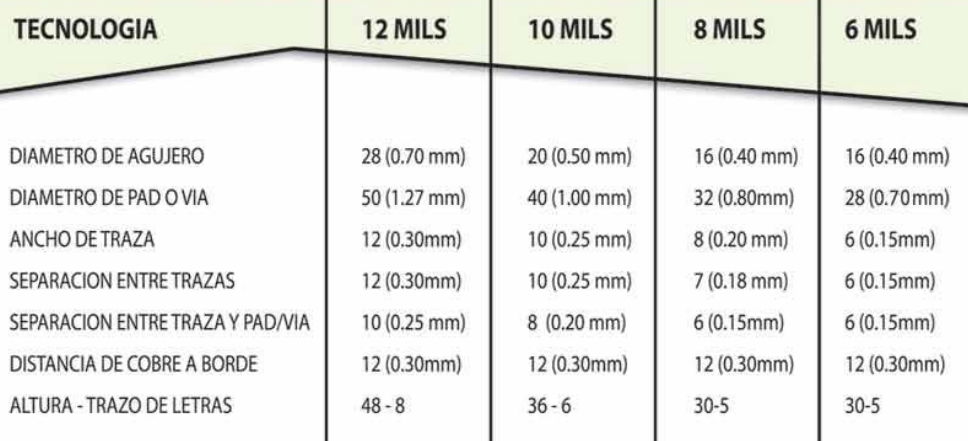
\includegraphics[width=110mm,keepaspectratio]{Figures/estandaresmayer.png}
	\caption{Estandares fijados por la empresa argentina Ernesto Mayer SA\protect\footnotemark .}
	\label{fig:mayerstandar}
\end{figure}


\footnotetext{\url{http://www.mayerpcb.com/informacion-tecnica.html}}

El resultado del diseño puede verse en la figura \ref{fig:PCBfrontt}, que es la cara superior de la placa donde se encuentran la mayoría de los componentes. 

\begin{figure}[!htb]
	\centering
	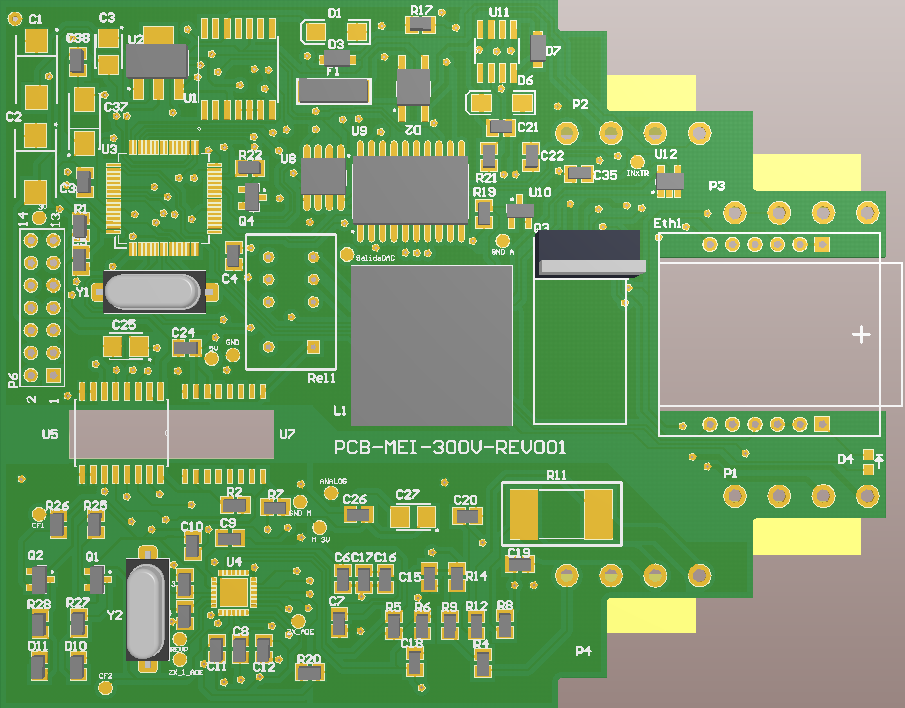
\includegraphics[width=110mm,keepaspectratio]{Figures/PCBfront.png}
	\caption{Imagen 3D de la parte frontal del PCB.}
	\label{fig:PCBfrontt}
\end{figure}

La cara inferior puede verse en la figura \ref{fig:PCBbackk}. Como esta cara se soldaría por refusión de una ola de estaño que viene de izquierda a derecha, tal como se ve en la imagen, se minimizó la cantidad de integrados en ella y se acomodaron los \textit{footprints} para que no queden puntos ciegos sin soldar.

\begin{figure}[!htb]
	\centering
	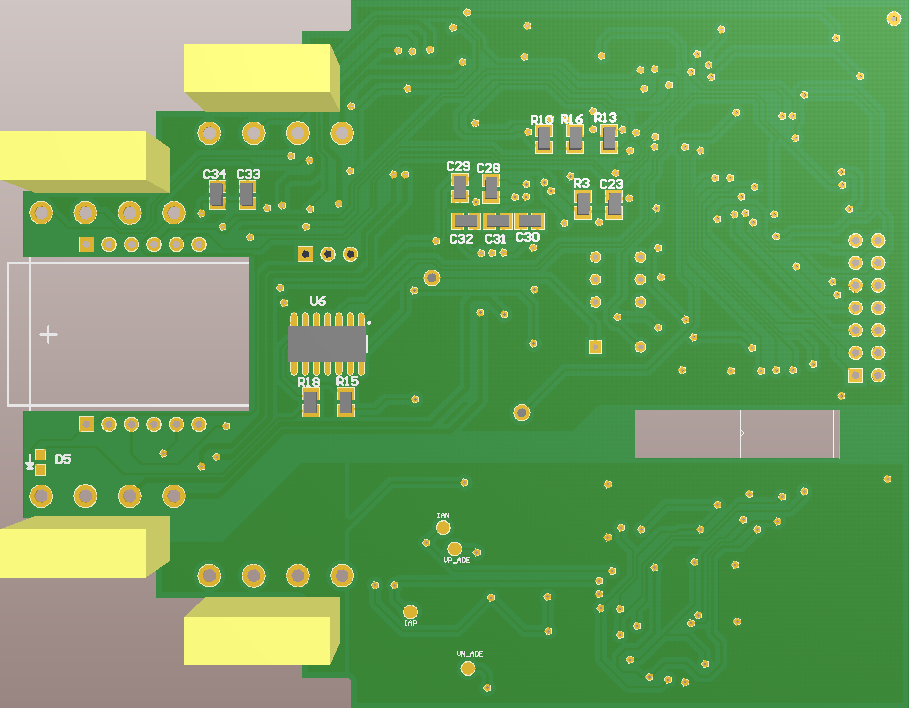
\includegraphics[width=110mm,keepaspectratio]{Figures/PCBback.png}
	\caption{Imagen 3D de la parte trasera del PCB.}
	\label{fig:PCBbackk}
\end{figure}



%%%%%%%%
\section{Diseño logrado}

Luego de finalizada la realización de la primera versión del circuito esquemático, se generaron los debidos archivos de fabricación y se envió a fabricar el PCB. Una vez obtenido el PCB la empresa SERVAIND S.A. se encargo del soldado y ensamblado de la electrónica sobre la placa. El resultado final puede verse en la figura  \ref{fig:proto1}. 

Debido a la inexperiencia en el uso del programa CAD de diseño se realizó un mal manejo del grid de trabajo en el esquemático. Algunos bloques de dispositivos fueron importados de bibliotecas externas y poseían medidas diferentes al grid de trabajo, por lo que el programa no detectaba como conexiones existentes a algunas conexiones realizadas. Este error fue trasladado al diseño del PCB por lo que las conexiones hechas no figuraban en la placa. Por ende las conexiones de alimentación del integrado de medición eran inexistentes como también la de los dos transistores discretos encargados de manejar el relé accionador y la señal de control.

%esto llevó a que líneas que aparecían conectadas en realidad no lo estuvieran, 


\begin{figure}[!htb]
	\centering
	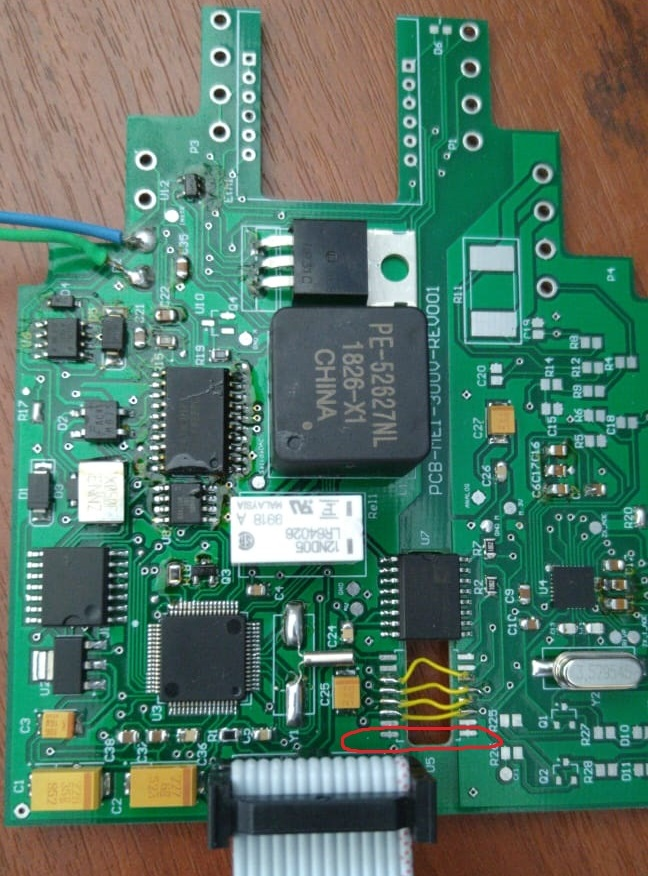
\includegraphics[width=80mm,keepaspectratio]{Figures/placaarmada1.jpeg}
	\caption{Primer PCB fabricado con conexiones arregladas.}
	\label{fig:proto1}
\end{figure}

Viendo las importantes faltantes en la placa, se procedió a corregir el diseño en el circuito esquemático y se decidió que se realizaría un segundo prototipo, que corregiría todos los problemas que presentó el primero. Para realizar las pruebas  de funcionamiento las conexiones faltantes se realizaron soldando cables en los terminales correspondientes, esto puede verse en la figura \ref{fig:parchess2}. Una vez asegurado el funcionamiento de los módulos se procedió a testear la placa.

\begin{figure}[!htb]
	\centering
	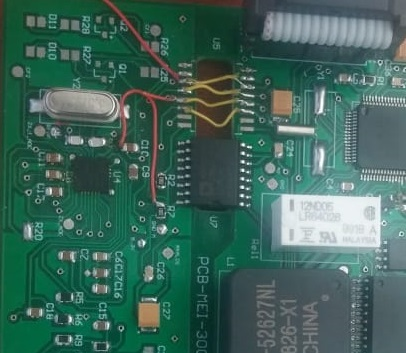
\includegraphics[width=80mm,keepaspectratio]{Figures/parche2.jpg}
	\caption{Soldado de cables para corregir el prototipo del PCB.}
	\label{fig:parchess2}
\end{figure}

El segundo prototipo desarrollado puede verse en la figura \ref{fig:Proto2}. Este prototipo es la versión final del trabajo desarrollado.

%todas las pistas se encuentran corregidas.

\begin{figure}[!htb]
	\centering
	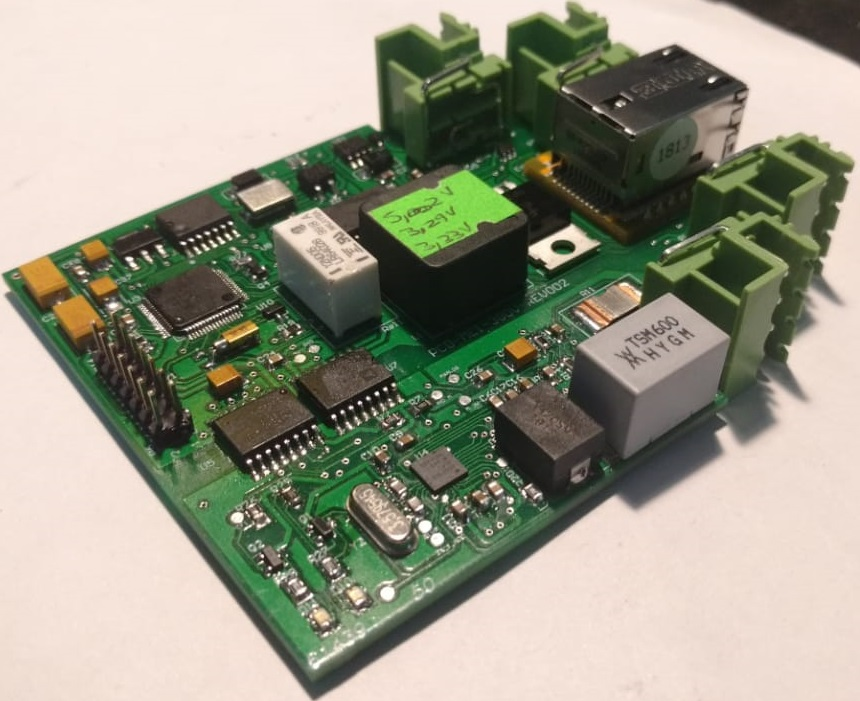
\includegraphics[width=\textwidth,keepaspectratio]{Figures/protofinal.jpeg}
	\caption{Segundo prototipo fabricado.}
	\label{fig:Proto2}
\end{figure}

%%%%%%%%%%


\section{Desarrollo de \textit{software}}

Una vez terminado el desarrollo de la primera versión del hardware se procedió a desarrollar un software capaz de controlar todos los dispositivos periféricos que fueron agregados a la placa. Inicialmente se comenzó a desarrollar la comunicación con el chip ADE 7953 y luego se procedió a realizar las diferentes comunicaciones. Por último se realizó el almacenamiento de datos en la EEPROM.

Si bien inicialmente no se planteó que estructura debía seguir el software, este fue el resultado de una evolución natural de los requisitos y exigencias del hardware. Luego de finalizar el software que daba funcionalidad a la electrónica se procedió a desarrollar una segunda parte de manejo de datos y configuración. Esta ultima parte desarrollada consta del manejo del protocolo Modbus y de dos menús de configuraciones, el de usuario y el de calibración.


\subsection{Software previos de base}
Se desarrolló durante la cursada de la Especialización un programa en lenguaje C para hacer uso de un circuito integrado wiznet w5500 con un microntrolador LPC4337. El wiznet w5500 es un controlador \textit{Ethernet} que maneja protocolo TCP/IP, comúnmente utilizado para realizar una conexión a internet de manera sencilla. Se pensó en el desarrollo de este programa para facilitar la implementación del futuro puerto \textit{Ethernet} del dispositivo.

También se habían desarrollado como parte de las materias de la Especialización programas simples de bucle infinito con interrupción para la introducción de sistemas operativos, uno de estos programas fue usado como base para la elaboración del programa final.


\subsection{Software del fabricante utilizados}

El fabricante Texas Instrument provee en su página web para la familia de microcontroladores MSP430 una conjunto de software de ejemplo, escritos en lenguaje C y altamente comentados, que utilizan los diferentes módulos del microcontrolador. Para el trabajo se usaron varios de estos ejemplos para realizar la implementación del programa del dispositivo.  

De los ejemplos escritos en C  se usaron principalmente los programas que controlan la interfaz UART,  los de manejo de memoria \textit{EEPROM} y los referidos al manejo del módulo ADC. El resto de los ejemplos sirvieron como referencia a la hora de configurar el microcontrolador.


%\begin{figure}[h]
%	\centering
%	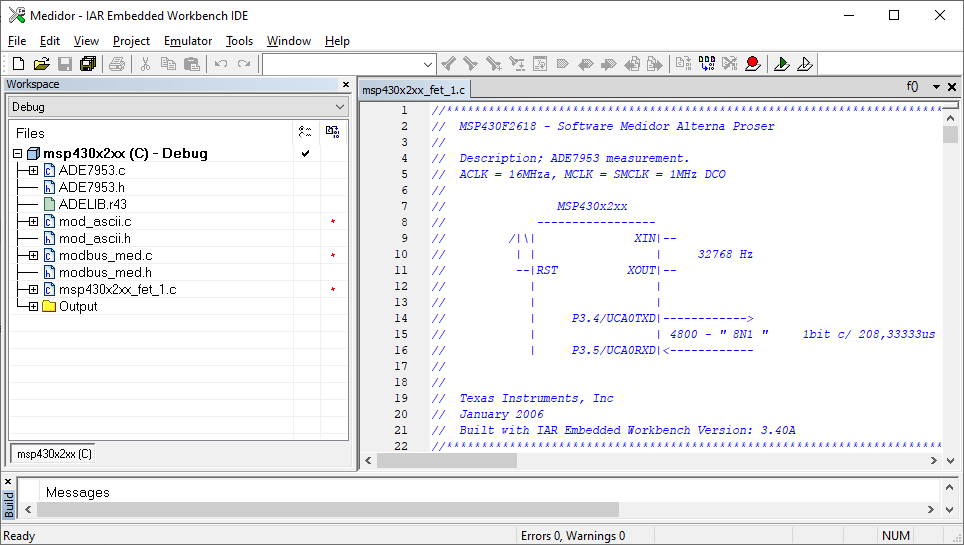
\includegraphics[width=110mm,keepaspectratio]{Figures/Embeddedworkbench.png}
%	\caption{Imagen del entorno de desarrollo.}
%	\label{fig:IARwindow}
%\end{figure}



\subsection{Especificaciones del software desarrollado}

Ante la necesidad de realizar un software robusto y de uso instrumental se deseaba implementar un FreeRTOS pero debido a limitaciones de memoria del microcontrolador resultaba inviable hacerlo, por lo que se decidió realizar un programa \textit{bare metal}.

El software realizado consiste en un bucle infinito controlado por tiempo (1 milisegundo) usando uno de los dos timers internos del microcontrolador. La principal tarea del programa es comunicarse constantemente con el integrado de medición ADE7953 y almacenar los datos de sus registros en la memoria local. Dentro del período de un milisegundo que dura el barrido del bucle se realizan otras tareas como comunicar datos a otros puertos, accionar el relé o cambiar los leds. En la figura \ref{fig:ProgFlux} se presenta un diagrama de flujo simplificado para entender el funcionamiento del programa.

\begin{figure}[h]
	\centering
	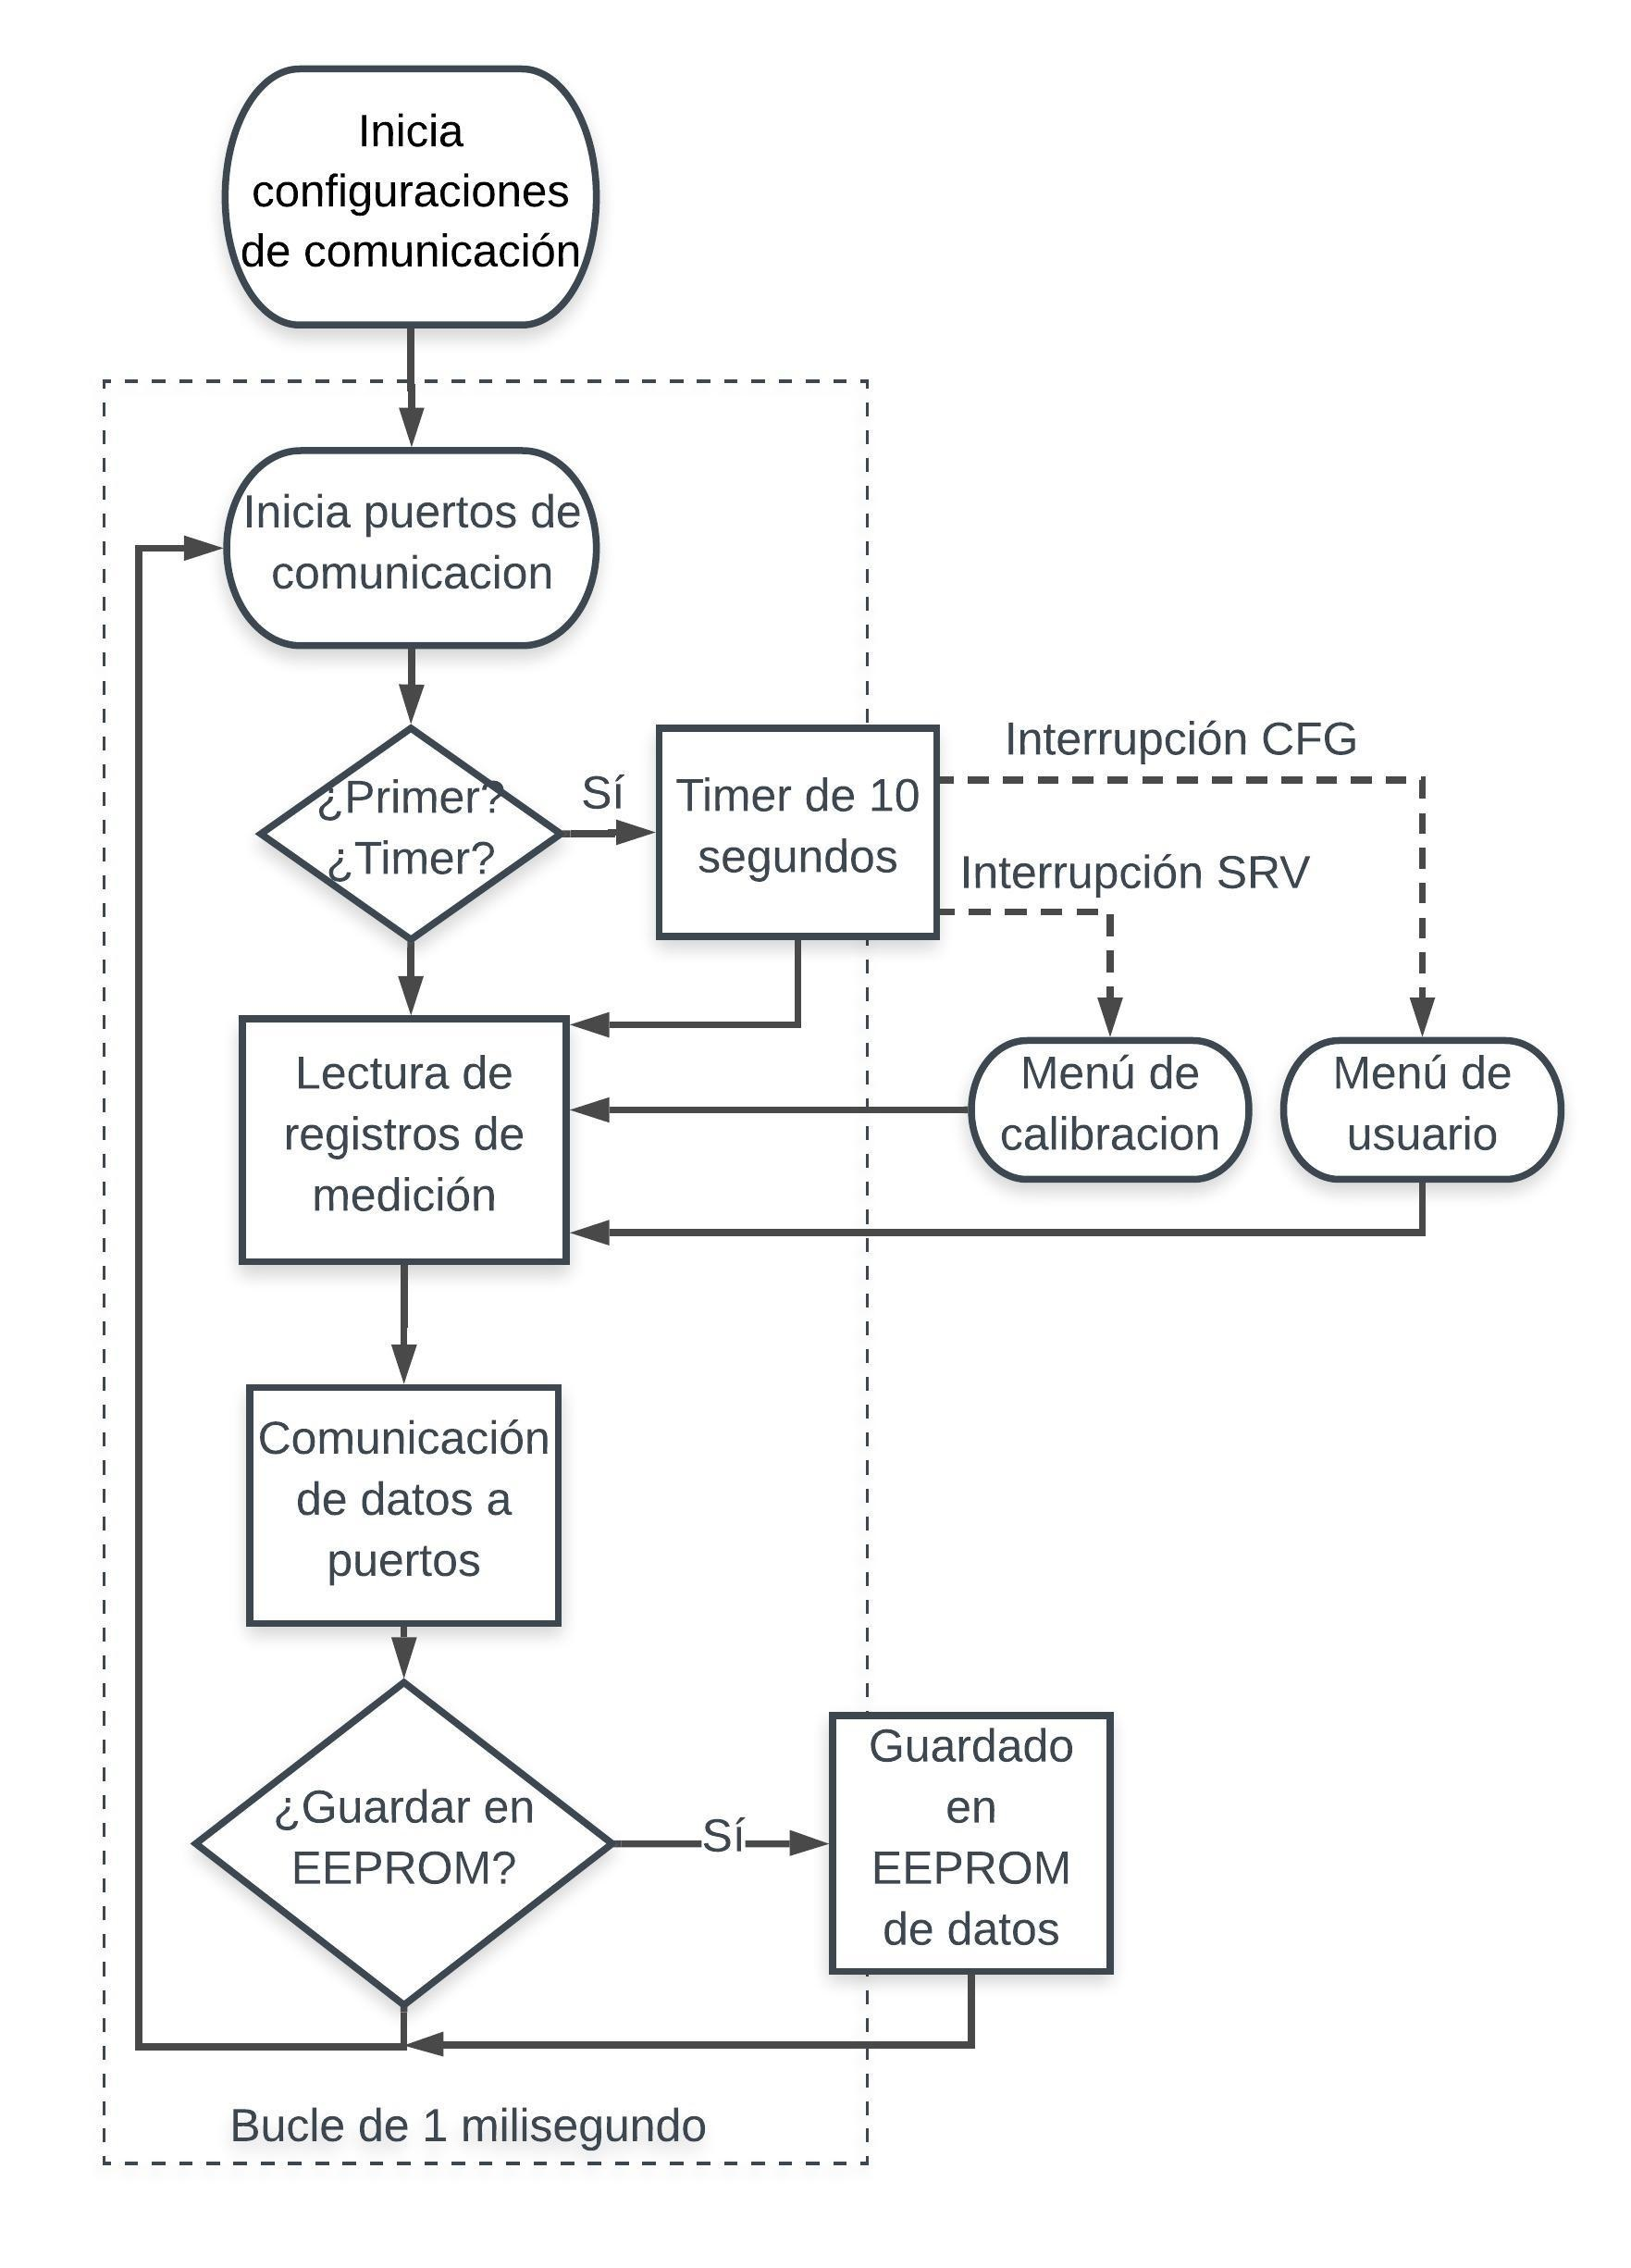
\includegraphics[width=110mm,keepaspectratio]{Figures/Diagramadeprograma.jpeg}
	\caption{Diagrama de flujo del programa.}
	\label{fig:ProgFlux}
\end{figure}


\subsubsection{Comunicación con el ADE7953}

La comunicación con el ADE7953 se realiza por UART por medio de un protocolo establecido por el fabricante del chip. Como la comunicación UART del chip está fijada en 4800 bps, cada frame que se le envía tiene un tiempo de 2,08 ms. El tiempo entre cada frame es de 0,2 ms a 4ms (el fabricante lo denomina como t1) como máximo y el tiempo de espera entre cada comunicación exitosa es de 6ms (el fabricante lo denomina como t2).

El ADE7953 tiene registros internos de 8, 16 y 24 bits donde almacena información de medición y de configuración para su funcionamiento. Estos registros son tanto de escritura como de lectura. La dirección  de registros de 8 bits puede verse en la tabla \ref{8biadcregis}.

Las operaciones de lectura con el ADE7953 pueden verse en la figura \ref{fig:ADEread}. Para leer un registro debe primeramente enviarse un byte de valor 0x35 y luego los bytes de la dirección del registro a leer, para luego recibir la cantidad de bytes según el tamaño del registro solicitado.

\begin{figure}[htb]
	\centering
	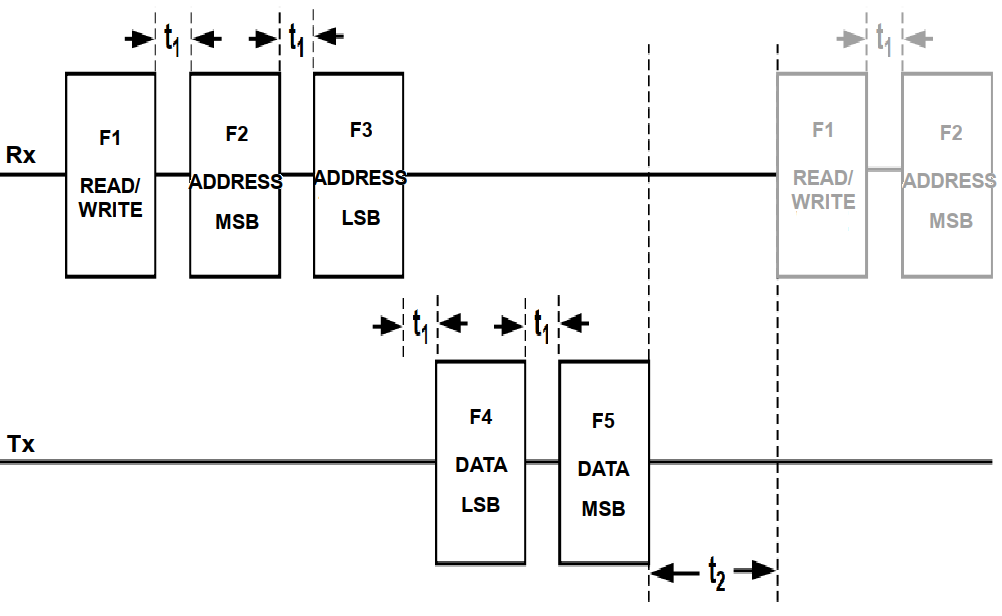
\includegraphics[width=\textwidth , keepaspectratio]{Figures/ade7uartread.png}
	\caption{Lectura por UART del ADE7953.}
	\label{fig:ADEread}
\end{figure}

Para la operación de escritura del ADE7953 debía enviarse un byte con el valor 0xCA, luego los bytes de la dirección a escribir y por último los datos en la misma cantidad de \textit{frames} que espacio del registro, como puede observarse en la figura \ref{fig:ADEwrite}.

\begin{figure}[htb]
	\centering
	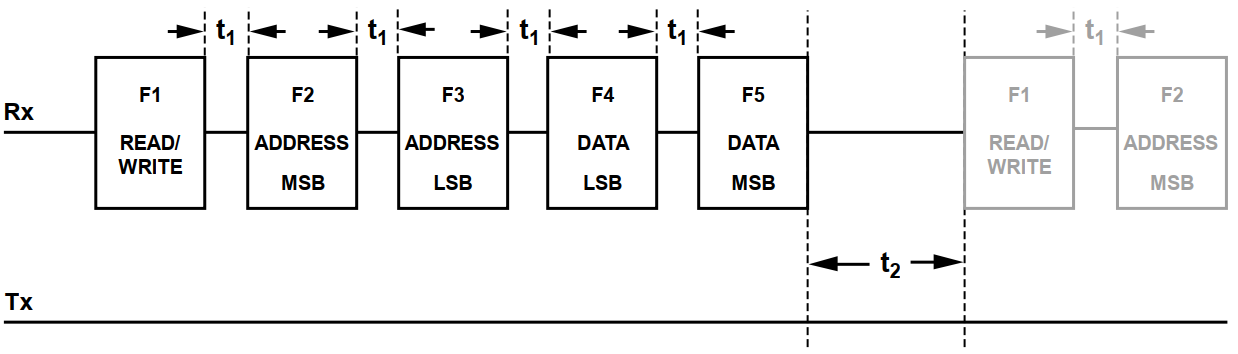
\includegraphics[width=110mm,keepaspectratio]{Figures/ade7uartwrite.png}
	\caption{Escritura por UART del ADE7953.}
	\label{fig:ADEwrite}
\end{figure}

Se configuró el programa de tal modo que lea los registros necesarios para monitorear la potencia eléctrica de la maquina donde se lo instale. Los registros que el programa lee y almacena son:

\begin{itemize}
\item AVA\_ 24 potencia aparente instantánea. 
\item AWATT\_ 24 potencia activa instantánea.
\item AVAR\_ 24 potencia reactiva instantánea. 
\item IA\_ 24 corriente instantánea.
\item V\_ 24 tensión instantánea.
\item IRMSA\_ 24 corriente RMS.
\item VRMS\_ 24 tensión RMS.
\item AENERGYA\_ 24 energía activa.
\item RENERGYA\_ 24 energía reactiva.
\item APENERGYA\_ 24  energía aparente.
\item VPEAK\_ 24 pico de tensión.
\item PFA\_ 16 factor de potencia.
\item Period\_ 16 registro de período.
\end{itemize}


El programa tarda aproximadamente un total de 241 ms en leer la totalidad de estos registros usando el protocolo elegido, por lo que queda un amplio margen para realizar otras operaciones.

%%%%%%%%%%%
%%%%%%%%%%
%%%%%%%%%

%\begin{table}[]
%\centering
%\caption[Registros 8 bit ADE79853]{Registros de 8 bit del ADE7953 como se los muestran en el \textit{datasheet} del fabricante.}
% Please add the following required packages to your document preamble:
% \usepackage{booktabs}
% Please add the following required packages to your document preamble:
% \usepackage{booktabs}
% Please add the following required packages to your document preamble:
% \usepackage[normalem]{ulem}
% \useunder{\uline}{\ul}{}

% Please add the following required packages to your document preamble:
% \usepackage[normalem]{ulem}
% \useunder{\uline}{\ul}{}
% Please add the following required packages to your document preamble:
% \usepackage{booktabs}
% \usepackage[normalem]{ulem}
% \useunder{\uline}{\ul}{}


% Please add the following required packages to your document preamble:
% \usepackage{booktabs}
% \usepackage[normalem]{ulem}
% \useunder{\uline}{\ul}{}

% Please add the following required packages to your document preamble:
% \usepackage{booktabs}
% \usepackage[normalem]{ulem}
% \useunder{\uline}{\ul}{}


% Please add the following required packages to your document preamble:
% \usepackage[normalem]{ulem}
% \useunder{\uline}{\ul}{}

% Please add the following required packages to your document preamble:
% \usepackage[normalem]{ulem}
% \useunder{\uline}{\ul}{}


% Please add the following required packages to your document preamble:
% \usepackage{booktabs}
% \usepackage[normalem]{ulem}
% \useunder{\uline}{\ul}{}
\begin{table}[]
\centering
\caption[Registros 8 bit ADE79853]{Registros de 8 bit del ADE7953\protect\footnotemark .}
\begin{tabular}{@{}llllll@{}}
\toprule
Address & Register Name  & R/W & Default & Type     & \begin{tabular}[c]{@{}l@{}}Register \\ Description\end{tabular}                                                                                             \\ \midrule
0x000   & SAGCYC         & R/W & 0x00    & Unsigned & Sag line cycles                                                                                                                                             \\
0x001   & DISNOLOAD      & R/W & 0x00    & Unsigned & \begin{tabular}[c]{@{}l@{}}No-load\\ detection\\ disable\end{tabular}                                                                                       \\
0x004   & LCYCMODE       & R/W & 0x40    & Unsigned & \begin{tabular}[c]{@{}l@{}}Line cycle \\ accumulation \\ mode \\ configuration\end{tabular}                                                                 \\
0x007   & PGA\_V         & R/W & 0x00    & Unsigned & \begin{tabular}[c]{@{}l@{}}Voltage channel \\ gain \\ configuration\\ (Bits{[}2:0{]})\end{tabular}                                                          \\
0x008   & PGA\_IA        & R/W & 0x00    & Unsigned & \begin{tabular}[c]{@{}l@{}}Current \\ Channel A\\ gain\\  configuration\\ (Bits{[}2:0{]})\end{tabular}                                                      \\
0x009   & PGA\_IB        & R/W & 0x00    & Unsigned & \begin{tabular}[c]{@{}l@{}}Current \\ Channel B\\ gain \\ configuration\\ (Bits{[}2:0{]})\end{tabular}                                                      \\
0x040   & WRITE\_PROTECT & R/W & 0x00    & Unsigned & \begin{tabular}[c]{@{}l@{}}Write protection\\ bits (Bits{[}2:0{]})\end{tabular}                                                                             \\
0x0FD   & LAST\_OP       & R   & 0x00    & Unsigned & \begin{tabular}[c]{@{}l@{}}Contains the \\ type (read \\ or write)\\ of the last \\ successful\\ communication \\ (0x35 =read;\\ 0xCA = write)\end{tabular} \\
0x0FF   & LAST\_RWDATA   & R   & 0x00    & Unsigned & \begin{tabular}[c]{@{}l@{}}Contains the data\\ from the last \\ successful 8-bit \\ register \\ communication\end{tabular}                                  \\
0x702   & Version        & R   & N/A     & Unsigned & \begin{tabular}[c]{@{}l@{}}Contains the\\  silicon version\\  number\end{tabular}                                                                           \\
0x800   & EX\_REF        & R/W & 0x00    & Unsigned & \begin{tabular}[c]{@{}l@{}}Reference input \\ configuration: \\ set  to 0 \\ for internal; \\ set to 1\\ for external\end{tabular}                          \\ \bottomrule
\end{tabular}
\label{8biadcregis}
\end{table}

\footnotetext{\url{https://www.analog.com/media/en/technical-documentation/data-sheets/ADE7953.pdf}}

%Va aqui

%\begin{table}[]
%\centering
%\caption[Registros 8 bit ADE79853]{Registros de 8 bit del ADE7953 como se los muestran en el \textit{datasheet} del fabricante.}


%\label{8biadcregis}
%\end{table}



\subsection{Funcionalidades del software}
El software maneja un menú por el cual una terminal puede comunicarse con el programa por medio de un puerto serie para realizar determinadas configuraciones. La comunicación debe iniciarse por el puerto RS232 del dispositivo.

Al iniciar el programa, dentro de los primeros 10 segundos se puede enviar caracteres en código ANSII. Si se envían las letras \textquotedblleft cfg\textquotedblright \ el programa inicia un menú, enviando caracteres con las opciones. Este menú puede verse en la figura  \ref{fig:serialmenu}.

El menú puede mostrar las variables que se están midiendo, puede configurar el puerto serie, modificar de qué variable depende la salida del bucle analógico y activar una alarma que acciona el relé dependiendo de una variable seleccionada.

%\begin{figure}[!htb]
%	\centering
%	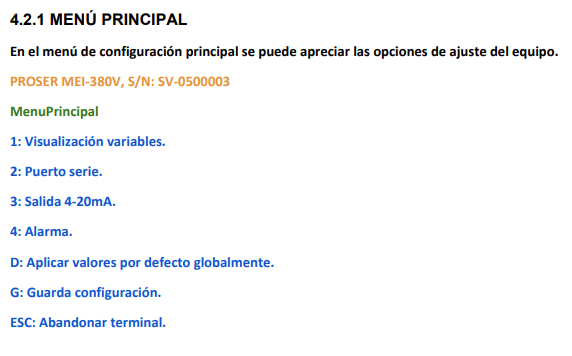
\includegraphics[width=110mm,keepaspectratio]{Figures/menumanual.png}
%	\caption{Menú serie en el manual.}
%	\label{fig:menumanual}
%\end{figure}

\begin{figure}[!htb]
	\centering
	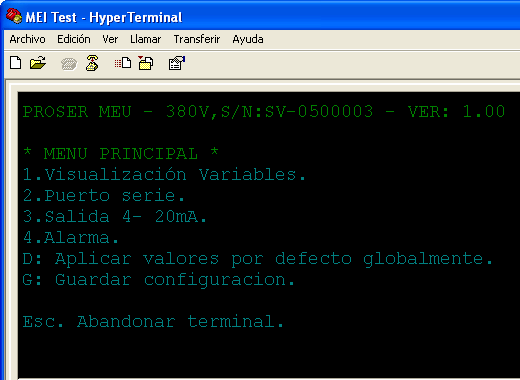
\includegraphics[width=110mm,keepaspectratio]{Figures/MenuUsuario1.png}
	\caption{Menú serie de configuración.}
	\label{fig:serialmenu}
\end{figure}

Se desarrolló el manejo de una salida para una conexión de lazo de corriente de 4 a 20 mA, que es un estándar en la industria para el control de procesos,  el programa puede hacer que esta salida sea proporcional a una variable de medición que puede seleccionarse en el menú serie de configuración.

El software almacena en la memoria del programa los valores de medición para poder comunicarlos ya sea por los puertos serie o el enlace de corriente.

Se guardan los valores de energía dentro de la EEPROM cada 40 segundos, se utiliza ese tiempo debido a que es el que tardaría el registro contador de energía en llenarse si se estuviera midiendo la máxima potencia posible.

\subsubsection{Protocolo Modbus }

El software que controla la placa maneja protocolo Modbus para comunicar registros internos en dos diferentes puertos de interfaces RS232 y RS485 según sean seleccionados. Para implementarlo se siguió como referencia el \textquotedblleft Modicon Modbus Protocol Reference Guide PI–MBUS–300\textquotedblright \ y un \textit{driver} libre, el Freemodbus.

El modo de acceder a los datos por Modbus es solicitando registros que el software maneja, la dirección de los registros puede verse en la tabla \ref{registrosmodbs}.

\begin{table}[h]
\caption[Registros Modbus en software]{Registros generados para la comunicación Modbus.}
\begin{tabular}{@{}lllll@{}}
\toprule
\begin{tabular}[c]{@{}l@{}}Dirección \\ del \\ Registro\end{tabular} & \begin{tabular}[c]{@{}l@{}}Número \\ del\\ parámetro\end{tabular} & Descripción                    & Unidades & Tipo de dato \\ \midrule
7001                                                                 & 1                                                                 & Tensión instantánea            & Volts    & Float 32     \\
7003                                                                 & 2                                                                 & Tensión rms                    & Volts    & Float 32     \\
7005                                                                 & 3                                                                 & Corriente instantánea          & Ampere   & Float 32     \\
7007                                                                 & 4                                                                 & Corriente rms                  & Ampere   & Float 32     \\
7009                                                                 & 5                                                                 & Potencia activa                & Watt     & Float 32     \\
7011                                                                 & 6                                                                 & Potencia reactiva              & VA       & Float 32     \\
7013                                                                 & 7                                                                 & Factor de potencia             & -        & Float 32     \\
7015                                                                 & 8                                                                 & Frecuencia                     & Hz       & Float 32     \\
7017                                                                 & 9                                                                 & Energía reactiva medida        & Joules   & Float 32     \\
7019                                                                 & 10                                                                & Energía activa total acumulada & kWh      & Float 32    
\end{tabular}
\label{registrosmodbs}
\end{table}

\subsubsection{Menú de calibración }

Además del menú de configuración, se desarrolló un segundo menú denominado menú de calibración, que puede verse en la figura \ref{fig:calibmenu}. Este menú también puede mostrar las variables que se encuentra midiendo el dispositivo, pero además permite realizar modificaciones sobre cómo se calculan las variables a medir. En este menú a diferencia del de configuración, en cada cambio que se realice se guarda en la memoria EEPROM para mantener los parámetros de calibración.

\begin{figure}[!htb]
	\centering
	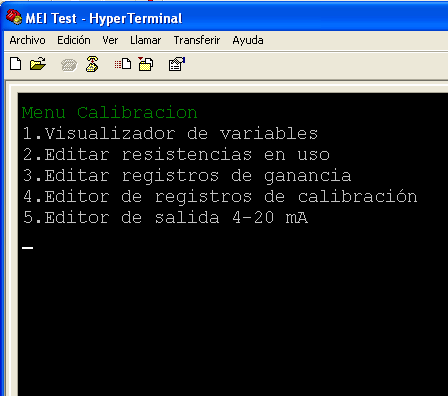
\includegraphics[width=110mm,keepaspectratio]{Figures/MenuCalib1.png}
	\caption{Menú de calibración.}
	\label{fig:calibmenu}
\end{figure}

El menú permite editar, según las resistencias soldadas en la placa, el cálculo de medición. Se puede especificar en la opción 2 del menú, que resistores posee el dispositivo para así realizar los cálculos correctos. En esta parte del desarrollo del software se parametrizan todas las variables que se involucran en el cálculo, por lo que se debe especificar qué valores de resistencia se involucran en la medición.

En la opción 3 del menú, se pueden editar las ganancias del chip de medición, el microcontrolador se comunica con el ADE7953 y configura el amplificador de ganancia programable según las opciones elegidas. Se puede variar qué ganancia usar para aumentar la precisión del cálculo. Ya que al variar la ganancia varían los rangos de medición, el menú muestra en esta sección que valores límite puede medir el dispositivo.

En la opción 4 del menú, se pueden editar los registros de calibración. Esta opción sirve para calibrar el dispositivo. Según que variable física se elija, debe inyectarse al dispositivo los valores que este solicite para que realice la calibración. El menú solicita 5 valores de medición para realizar los cálculos. Un documento que detalla y resume los procesos de calibración fue realizado y enviado a la empresa.

La última opción del menú  permite variar  los valores de cálculo de la salida 4-20 mA de manera manual. La opción permite variar la corriente que el software interpreta como mínima o también la que interpreta como máxima, para adecuarse al valor real.


